\section{Reconstruction des jets}\label{chapter-JERC-section-jets_reco}

q,g --> jet dans détecteur


\subsection{Algorithmes de reconstruction}\label{chapter-JERC-section-jets_reco-subsec-algo}
Dans la section~\ref{chapter-JERC-section-jets}, nous avons vu que les radiations de partons sont plus importantes pour de basses énergies (limite infrarouge) ou pour un parton radié colinéaire au parton initial (limite colinéaire).
Afin de conserver des prédictions de QCD vérifiables sur des jets réels, les algorithmes de reconstruction doivent être insensibles à l'ajout d'une particule de basse énergie ou au partage d'une particule en deux particules d'énergies inférieures. C'est ce que l'on appelle l'insensibilité IRC, pour \emph{InfraRed and Colinear}.


anti-\kT

M. Cacciari, et al. The anti-k t jet clustering algorithm. JHEP, 04 :063, 2008.
doi :10.1088/1126-6708/2008/04/063. 0802.1189.

\begin{equation}
d_{ij} = \min(\frac{1}{\pT^2_i}, \frac{1}{\pT^2_j}) \frac{\Delta R^2_{ij}}{R^2}
\end{equation}
voir le cours de GGrenier

produit des jets de forme régulière, plutôt conique

moins sensible aux perturbations dues aux partons spectateurs

regroupement autour des particules de plus haute énergie en utilisant les écarts angulaires

moins proche de l'évolution du parton shower

\begin{figure}
\centering
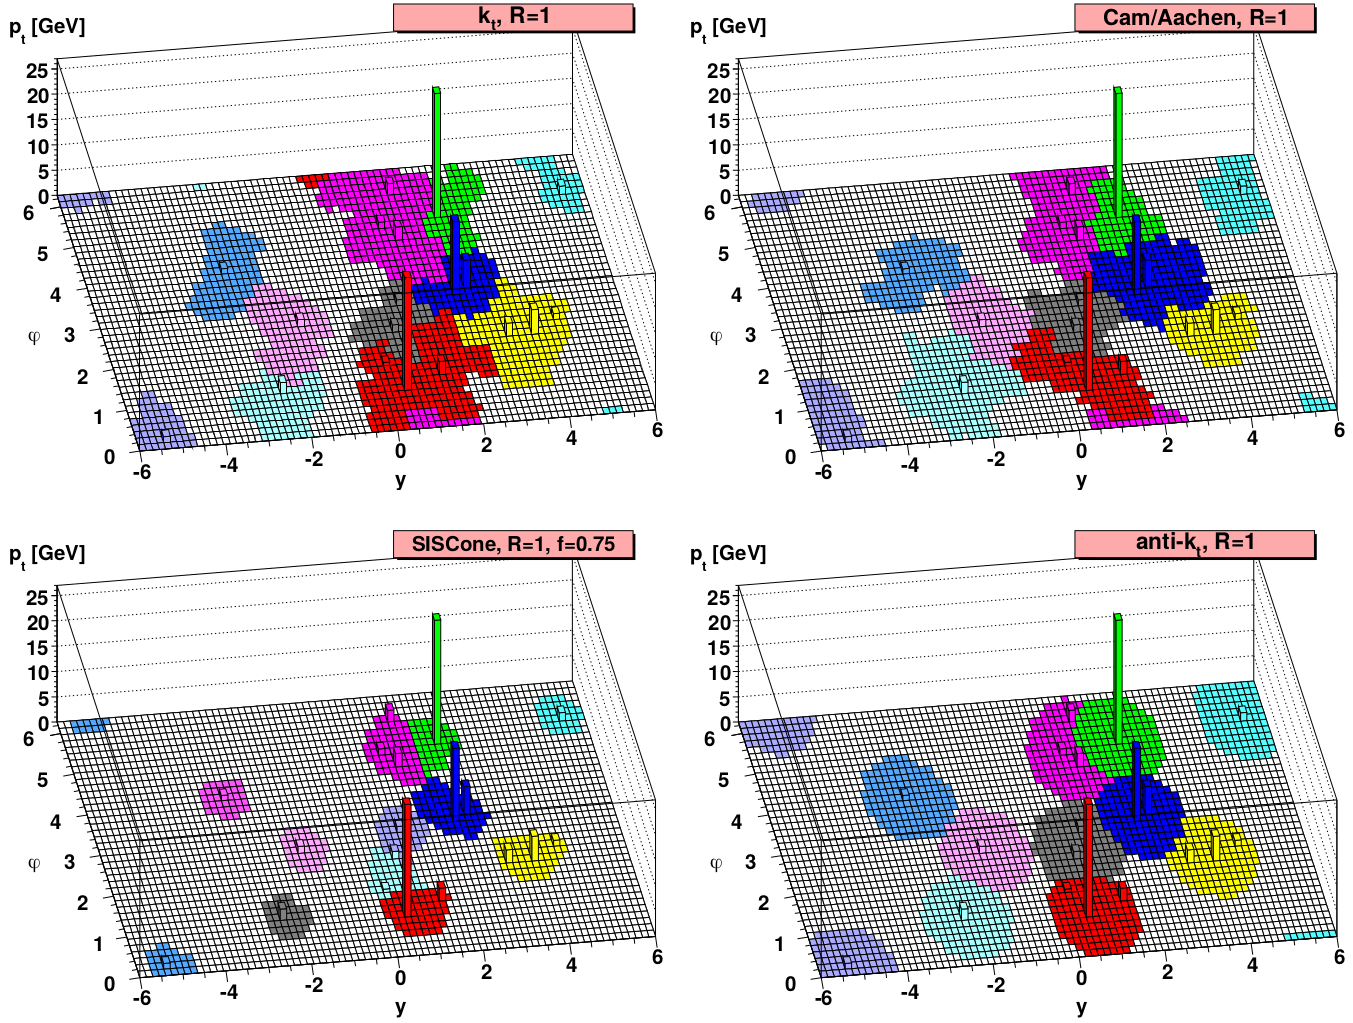
\includegraphics[width=.8\textwidth]{\PhDthesisdir/contents/chapter-JERC/reconstruction_des_jets/forme_des_jets.png}
\caption{Formes des jets reconstruits à partir de différents algorithmes pour un même événement. En haut à gauche, \kT; en haut à droite, C/A; en bas à gauche, SISCone; en bas à droite, anti-\kT. L'algorithme anti-\kT\ permet d'obtenir des jets de forme régulière, conique.}
\end{figure}
\begin{figure}
\centering
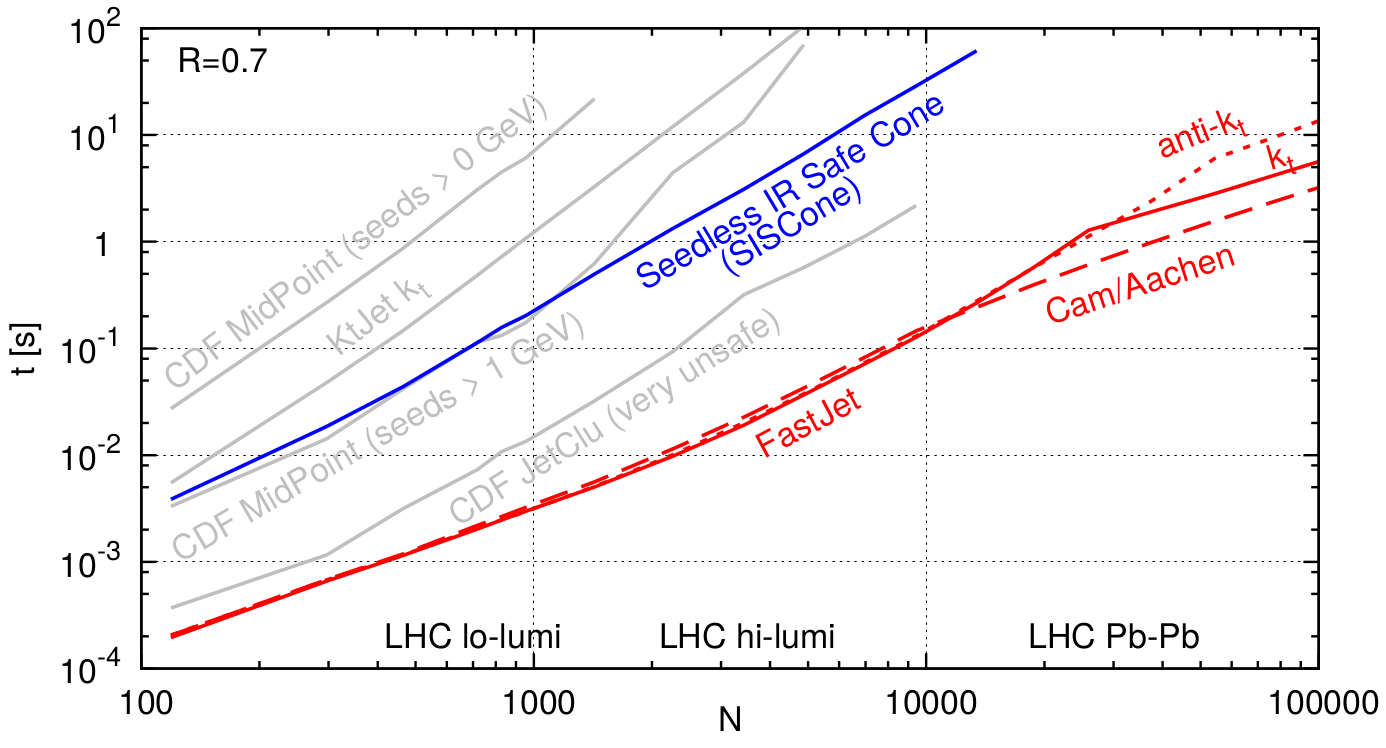
\includegraphics[width=.6\textwidth]{\PhDthesisdir/contents/chapter-JERC/reconstruction_des_jets/temps_de_calcul.png}
\caption{Temps de reconstruction d'un empilement d'un événement di-jets avec $N$ événements ne produisant que des jets de bas \pT\ pour différents algorithmes de reconstruction des jets.} % 50 GeV
\end{figure}

\subsection{Identification des jets dans CMS}\label{chapter-JERC-section-jets_reco-subsec-jetID}
quels critères?

\subsection{Saveur des jets}\label{chapter-JERC-section-jets_reco-subsec-flavor}
b-tagging

\begin{figure}
\centering
\begin{tikzpicture}[scale=1.5]
\def\trackerrin{.100}
\def\trackerrout{1.185}
\def\trackercolor{ltcolorgray1}

\def\ECALrin{1.290}
\def\ECALrout{1.811}
\def\ECALcolor{ltcolorgreen1}

\def\HCALrin{1.812}
\def\HCALrout{2.854}
\def\HCALcolor{ltcoloryellow3}

\def\Solenrin{2.950}
\def\Solenrout{3.800}
\def\Solencolor{ltcolorgray2}

\def\ironryrina{3.850}
\def\ironryrouta{4.000}
\def\muonrina{4.020}
\def\muonrouta{4.400}
\def\ironryrinb{4.420}
\def\ironryroutb{4.880}
\def\muonrinb{4.905}
\def\muonroutb{5.285}
\def\ironryrinc{5.300}
\def\ironryroutc{5.960}
\def\muonrinc{5.975}
\def\muonroutc{6.355}
\def\ironryrind{6.375}
\def\ironryroutd{6.980}
\def\muonrind{7.000}
\def\muonroutd{7.380}
\def\muoncolor{ltcoloryellow1}
\def\ironrycolor{ltcolorred2}

\def\printele#1{
\draw [thick, ltcolorred] (0,0) arc (#1-90:#1-90+27:3) coordinate (eledeposit);
\draw [ltcolorred] (#1-5:1.25) node {\ele};
}
\def\printmu#1{
\draw [thick, ltcolorblue] (0,0) arc (#1-90:#1-90+33:6) arc (#1-90+33:#1-90:-12) node{\mu};
\draw [ltcolorblue] (#1-7:1.5) node {\mu};
}

\def\printantiele#1{
\draw [thick, ltcolorred] (0,0) arc (#1-90:#1-90-27:-3) coordinate (eledeposit);
\draw [ltcolorred] (#1-7:1.5) node {\ele};
%\draw [ltcolorred4, ultra thick] (eledeposit)--+(#1+25:\ECALrout);
}
\def\printantimu#1{
\draw [thick, ltcolorblue] (0,0) arc (#1-90:#1-90-33:-6) arc (#1-90-33:#1-90:12);
\draw [ltcolorblue] (#1-7:1.5) node {\mu};
}

\def\printtauh#1{
\draw [thick, ltcolorgreen4] (0,0) arc (#1-90:#1-90+11:10) ;
\draw [thick, ltcolorgreen4] (0,0) arc (#1-90:#1-90+6:20) ;
\draw [thick, ltcolorgreen4] (0,0) arc (#1-90:#1-90-11:-10) ;
\draw [ltcolorgreen4] (#1-12:1.5) node {\tauh};
}
\def\printantitauh#1{
\draw [thick, ltcolorgreen4] (0,0) arc (#1-90:#1-90-11:-10) ;
\draw [thick, ltcolorgreen4] (0,0) arc (#1-90:#1-90-6:-20) ;
\draw [thick, ltcolorgreen4] (0,0) arc (#1-90:#1-90+11:10) ;
\draw [ltcolorgreen4] (#1-12:1.5) node {\tauh};
}

\def\printjetnolabel#1{
\draw [thick, ltcolororange] (0,0) arc (#1-90+10:#1-90+22+10:5) ;
\draw [thick, ltcolororange] (0,0) arc (#1-90+5:#1-90+12+5:10) ;
\draw [thick, ltcolororange] (0,0) arc (#1-90:#1-90-22:-5) ;
\draw [thick, ltcolororange] (0,0) arc (#1-90:#1-90+6:20) ;
\draw [thick, ltcolororange] (0,0) arc (#1-90+5:#1-90+8+5:10) ;
\draw [thick, ltcolororange] (0,0) arc (#1-90:#1-90-11:-10) ;
\draw [thick, ltcolororange] (0,0) arc (#1-90:#1-90+11:10) ;
}

\def\printjet#1{
\printjetnolabel{#1}
\draw [ltcolororange] (#1-25:.5) node {jet};
}

\def\printjetfake#1{
\printjet{#1}
\draw [thick, ltcolorgreen4] (0,0) arc (#1-90:#1-90+11:10) ;
\draw [thick, ltcolorgreen4] (0,0) arc (#1-90:#1-90+6:20) ;
\draw [thick, ltcolorgreen4] (0,0) arc (#1-90:#1-90-11:-10) ;
\draw [ltcolorgreen4] (#1-17:1.5) node {f.\tauh};
}

\def\printdeposit#1#2#3#4{
\fill [#1] (#2-2:#3) arc (#2-2:#2+2:#3) -- (#2+2:#4) arc (#2+2:#2-2:#4) ;
}

\def\printECALdeposit#1#2{\printdeposit{#1}{#2}{\ECALrin}{\ECALrout}}
\def\printHCALdeposit#1#2{\printdeposit{#1}{#2}{\HCALrin}{\HCALrout}}

\def\printtauhdeposit#1{
\printHCALdeposit{ltcoloryellow4}{#1+3}
\printHCALdeposit{ltcoloryellow4}{#1+5}
\printHCALdeposit{ltcoloryellow4}{#1-5}
}

\def\printjetdeposit#1{
\printHCALdeposit{ltcoloryellow4}{#1+3}
\printHCALdeposit{ltcoloryellow4}{#1+5}
\printHCALdeposit{ltcoloryellow4}{#1-5}
\printHCALdeposit{ltcoloryellow4}{#1+21}
\printHCALdeposit{ltcoloryellow4}{#1+11}
\printHCALdeposit{ltcoloryellow4}{#1-11}
}

\def\printMuChSigA#1#2{
\fill [red] (#1-7.5+20*#2:\muonrina) arc (#1-7.5+20*#2:#1+7.5+20*#2:\muonrina) -- (#1+7.5+20*#2:\muonrouta) arc (#1+7.5+20*#2:#1-7.5+20*#2:\muonrouta) ;
}
\def\printMuChSigB#1#2{
\fill [red] (#1-7.5+20*#2:\muonrinb) arc (#1-7.5+20*#2:#1+7.5+20*#2:\muonrinb) -- (#1+7.5+20*#2:\muonroutb) arc (#1+7.5+20*#2:#1-7.5+20*#2:\muonroutb) ;
}
\def\printMuChSigC#1#2{
\fill [red] (#1-7.5+20*#2:\muonrinc) arc (#1-7.5+20*#2:#1+7.5+20*#2:\muonrinc) -- (#1+7.5+20*#2:\muonroutc) arc (#1+7.5+20*#2:#1-7.5+20*#2:\muonroutc) ;
}
\def\printMuChSigD#1#2{
\fill [red] (#1-7.5+20*#2:\muonrind) arc (#1-7.5+20*#2:#1+7.5+20*#2:\muonrind) -- (#1+7.5+20*#2:\muonroutd) arc (#1+7.5+20*#2:#1-7.5+20*#2:\muonroutd) ;
}

\foreach\jetangle in {120,-145}{
\printbigjetnolabel{\jetangle}
\draw (\jetangle:2.5) node {jet} ;
}

\def\Bjetangle{30}
\def\Bhaddronangle{5}
\def\Bhaddronflight{.75}

\def\CurrentVertex{(\Bhaddronangle:\Bhaddronflight)}

\draw [thick, dotted] (0,0) -- \CurrentVertex ;

{
\def\jetcolor{ltcolorred}
\printjetnolabel{\Bjetangle}
\draw [\jetcolor] (\Bjetangle:2)+(1.5,.75) node {traces déplacées};
}
\begin{scope}
\clip circle (\Solenrin);
\printantimuonnolabel{\Bjetangle}
\end{scope}

\draw [\muoncolor] (\Bjetangle:4) +(0,{-2*\baselineskip}) node {lepton chargé};

\draw (\Bjetangle:4) + (-.125,-.5) circle (1.125);
\draw [-latex] (\Bjetangle:4) + (-.125,-1.625) --+ (-.125,-2) node [below] {jet de saveur lourde};

\draw (0,0) node [left] {PV} ;
\draw \CurrentVertex node [below right] {SV} ;

\fill (0,0) circle (2pt);
\fill \CurrentVertex circle (2pt);

\draw [dashed] \CurrentVertex --+ (\Bjetangle:-.8);

\draw [red, latex-latex] (0,0)--+ (-90+\Bjetangle:{\Bhaddronflight*sin(\Bjetangle-\Bhaddronangle)}) node [below right] {IP};
\end{tikzpicture}
\end{figure}